%%%%%%%%%%%%%%%%%%%%%%%%%%%%%%%%%%%%%%%%% 
% Masters Thesis 
%
% This template is based on templates by:
% - Mario Román (https://github.com/mroman42)
% - Steve Gunn (http://users.ecs.soton.ac.uk/srg/softwaretools/document/templates/)
% - Sunil Patel (http://www.sunilpatel.co.uk/thesis-template/)
%
% Modifications done by Pedro Bonilla. 
% Template license:
% CC BY-NC-SA 3.0 (http://creativecommons.org/licenses/by-nc-sa/3.0/)
%
%%%%%%%%%%%%%%%%%%%%%%%%%%%%%%%%%%%%%%%%%

%----------------------------------------------------------------------------------------
%	PACKAGES AND OTHER DOCUMENT CONFIGURATIONS
%----------------------------------------------------------------------------------------

\documentclass[
12pt,
% oneside, % Two side (alternating margins) for binding by default, uncomment to switch to one side
english, % ngerman for German
singlespacing, % Single line spacing, alternatives: onehalfspacing or doublespacing
%draft, % Uncomment to enable draft mode (no pictures, no links, overfull hboxes indicated)
%nolistspacing, % If the document is onehalfspacing or doublespacing, uncomment this  to set spacing in lists to single
%liststotoc, % Uncomment to add the list of figures/tables/etc to the table of contents
%toctotoc, % Uncomment to add the main table of contents to the table of contents
%parskip, % Uncomment to add space between paragraphs
%nohyperref, % Uncomment to not load the hyperref package
headsepline, % Uncomment to get a line under the header
%chapterinoneline, % Uncomment to place the chapter title next to the number on one line
%consistentlayout, % Uncomment to change the layout of the declaration, abstract and acknowledgements pages to match the default layout
]{MastersDoctoralThesis} % The class file specifying the document structure


\usepackage[utf8]{inputenc} % Required for inputting international characters
\usepackage[T1]{fontenc} % Output font encoding for international characters
\usepackage{stmaryrd}
\usepackage{mathpazo} % Use the Palatino font by default
\usepackage[font=itshape]{quoting} 
\usepackage[toc,page]{appendix}
\usepackage[nogin]{Sweave}
\usepackage{pdfpages}
\usepackage[backend=biber,style=numeric]{biblatex} 
\usepackage[activate={
  true,nocompatibility},final,tracking=true,kerning=true,spacing=true,factor=1100,stretch=10,shrink=10]{microtype}
\usepackage{eso-pic}
\usepackage[autostyle=true]{csquotes} 

\addbibresource{./example.bib} % The filename of the bibliography



%----------------------------------------------------------------------------------
%	MARGIN SETTINGS
%----------------------------------------------------------------------------------

\geometry{
	paper=a4paper, % Change to letterpaper for US letter
	inner=2.5cm, % Inner margin
	outer=3.8cm, % Outer margin
	bindingoffset=.5cm, % Binding offset
	top=1.5cm, % Top margin
	bottom=1.5cm, % Bottom margin
	%showframe, % Uncomment to show how the type block is set on the page
}

%----------------------------------------------------------------------------------
%	THESIS INFORMATION AND METADATA
%----------------------------------------------------------------------------------
\usepackage[allcolors=myred]{hyperref}

\author{Pedro Bonilla Nadal}
\newcommand{\miTitulo}{Categories in Homotopy Type Theory\\\xspace}
\newcommand{\miNombre}{Pedro Bonilla Nadal\xspace}
\newcommand{\miGrado}{Máster en Matemáticas y Aplicaciones}
\newcommand{\miFacultad}{Facultad de Ciencias}
\newcommand{\miUniversidad}{Universidad Autónoma de Madrid}
% Añadir tantos tutores como sea necesario separando cada uno de ellos
% mediante el comando `\\\medskip` y una línea en blanco
\newcommand{\miTutor}{
Dr. Ángel González Prieto  \\ \emph{Departamento - Universidad}}
\newcommand{\miCurso}{2020-2021\xspace}
\newcommand{\misPalabrasClave}{HOTT, McLane}


\hypersetup{pdfinfo={
            Title={\miTitulo},
            Author={\miNombre},
            Director1={Dr. Ángel González Prieto},
            Director2={Federico Cantero Morán},
            Ndirectores={2}
            Tipo={TFM},
            Curso={\miCurso},
            MSC={ MSC2020},
            Palabrasclave={\misPalabrasClave},
          }
        }

\AtBeginDocument{
\hypersetup{pdftitle=\miTitulo} 
\hypersetup{pdfauthor=\miNombre}
\hypersetup{pdfkeywords=\misPalabrasClave}
}

%%%%%%%%%%%%%%%%%%%%%%%%%%%%%%%%%%%%%%%%%%%%%%%%%%%%%%%%%%%%%%%%%%%%%%%%%%%%%%%%%%%


%----------------------------------------------------------------------------------
%          OTHER IMPORTS
%----------------------------------------------------------------------------------


\usepackage[utf8]{inputenc}
%\usepackage[british]{babel}
\usepackage{caption}
\usepackage{adjustbox}
\usepackage{enumitem}
\usepackage{boldline}
\usepackage{amssymb, amsmath}
\usepackage{amsthm}
\usepackage{soul}
\usepackage{upgreek}
\usepackage{wrapfig}
\usepackage{mathtools}
\usepackage{epigraph}
\usepackage{algorithm}
\usepackage[noend]{algpseudocode}
\usepackage{soul}
\usepackage{graphicx}
\usepackage{mathrsfs}
\usepackage{xcolor}


\usepackage{tikz-cd}
\tikzcdset{arrow style=tikz, diagrams={>=stealth}}

\newtheorem{theorem}{Theorem}[section]
\newtheorem{corollary}{Corollary}[theorem]
\newtheorem{thesis}[theorem]{Thesis}
\newtheorem{lemma}[theorem]{Lemma}
\theoremstyle{definition}
\newtheorem{definition}{Definition}[section]
\newtheorem{proposition}{Proposition}[section]
\newtheorem{example}{Example}[section]
\newtheorem{remark}{Remark}[section]
\newcommand\myeq{\stackrel{\mathclap{\normalfont\mbox{?}}}{=}}

\newcommand{\R}{\mathbb{R}}
\newcommand{\N}{\mathbb{N}}
\newcommand{\dom}{\operatorname{dom}}
\newcommand{\codom}{\operatorname{codom}}
\newcommand{\hom}{\operatorname{hom}}

\begin{document}
\frontmatter
% TODO: Añadir cuando 
% 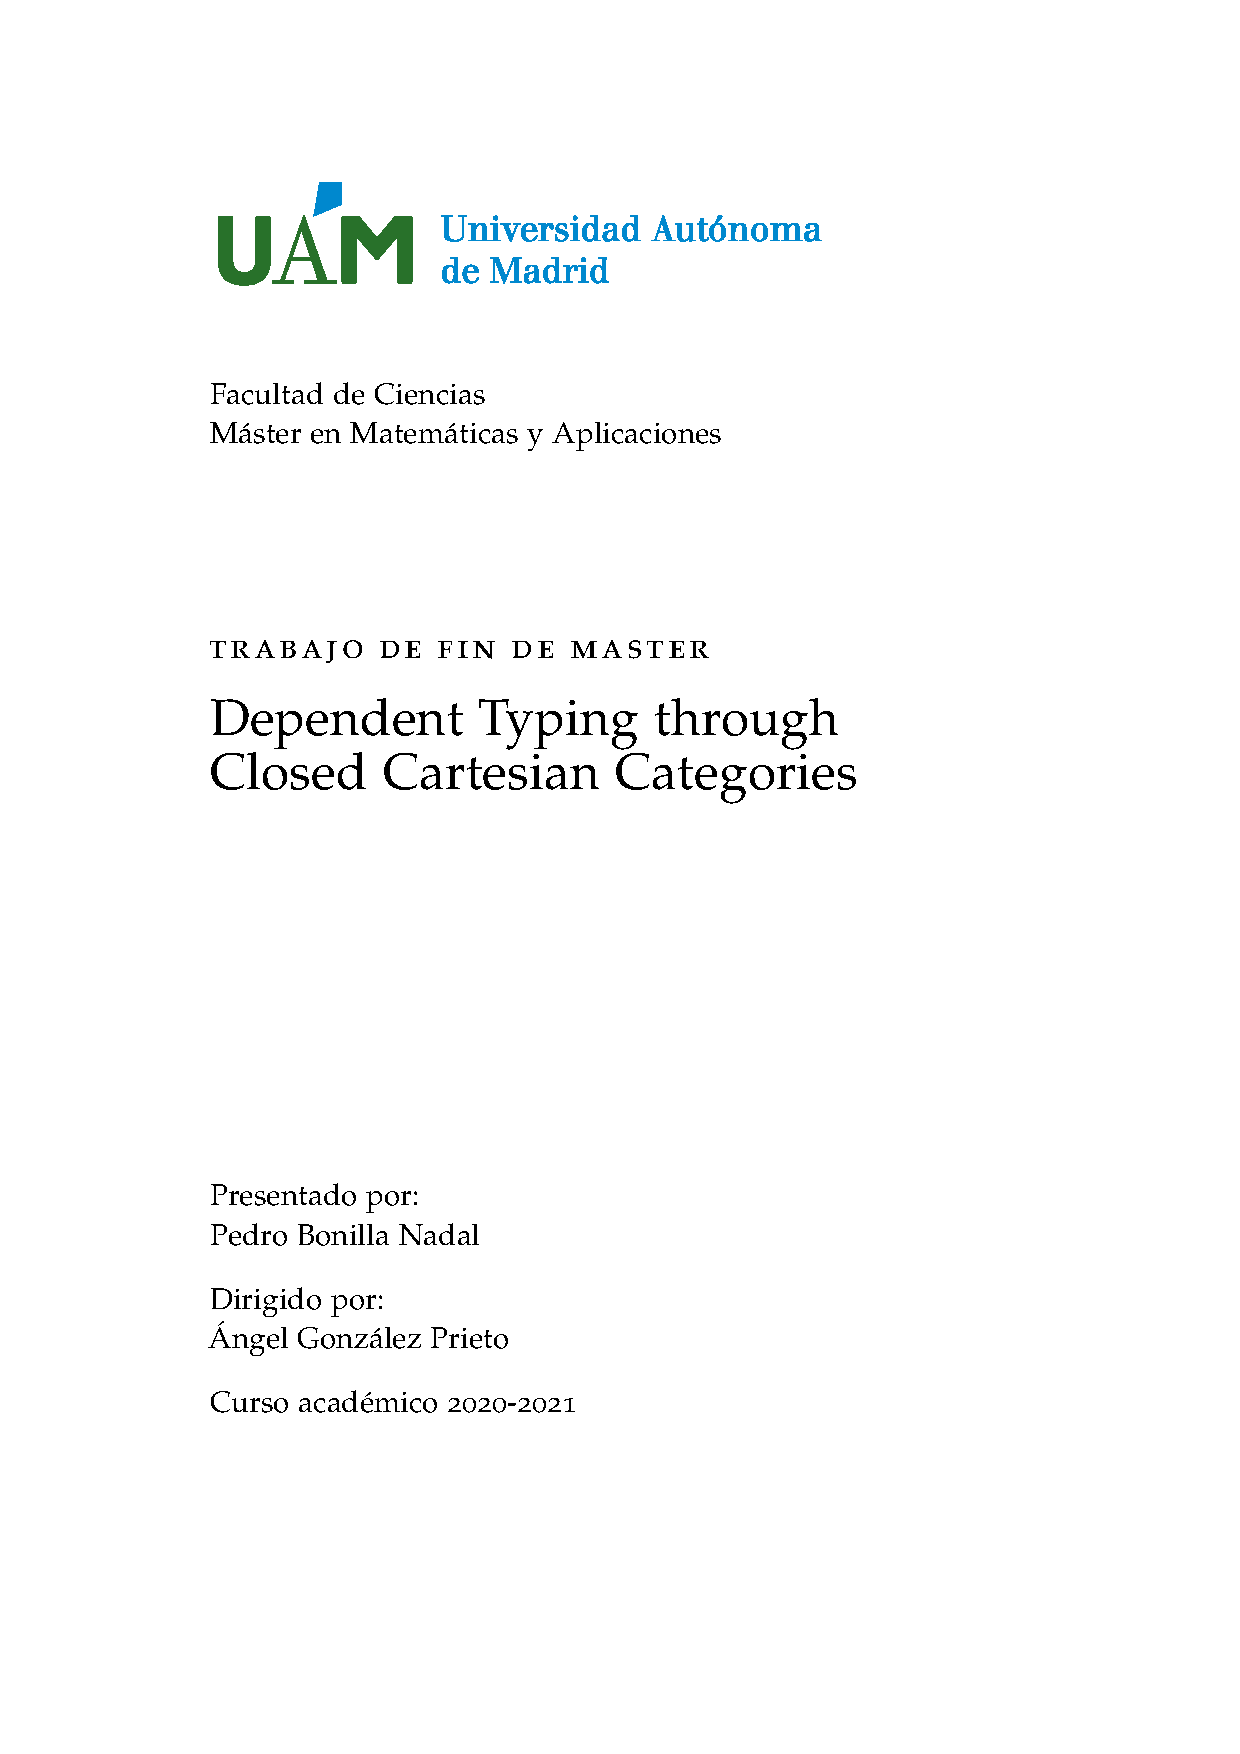
\includepdf{img/portada.pdf}
% \cleardoublepage
% !TeX root = ../libro.tex
% !TeX encoding = utf8

%*******************************************************
% Little Dirty Titlepage
%*******************************************************

\thispagestyle{empty}

\begin{center}
  {\small TODO: incluir portada oficial}
  \large  

  \vspace*{\stretch{1}}

  \begingroup
  \huge{\miTitulo} \\
  {\small (Título provisional - busca uno definitivo - probablemente en mayo)}
  \bigskip
  
  \endgroup

  \textrm{\miNombre}

  \vspace{\stretch{5}}

\end{center}  

\newpage
\thispagestyle{empty}

\hfill

\vfill

\miNombre\ \textit{\miTitulo}.

Master's thesis.

Academic year \miCurso.\\

\begin{minipage}[t]{0.25\textwidth}
  \flushleft
  \textbf{Thesis\\ supervisor}
\end{minipage}
\begin{minipage}[t]{0.40\textwidth}
  \flushleft
  \miTutor
\end{minipage}
\begin{minipage}[t]{0.35\textwidth}
  \flushright
  \miGrado
  \medskip

  \miUniversidad
\end{minipage}
\begin{flushleft}
\end{flushleft}

\endinput

% % !TeX root = ../libro.tex
% !TeX encoding = utf8
%
%*******************************************************
% Declaración de originalidad
%*******************************************************

\thispagestyle{empty}

\hfill\vfill

\textsc{Statement of Originality}\\\bigskip

D. \miNombre \\\medskip

 
I explicitly declare that the work presented as a Master's thesis (TFM) corresponding to the academic year \miCurso, is original, understood in the sense that it has not used sources for the elaboration of the work without citing them properly.

\medskip

Madrid, \today.
\begin{flushleft} 
Fdo: \miNombre 

\end{flushleft}

\vfill

\cleardoublepage
\endinput

% % !TeX root = ../libro.tex
% !TeX encoding = utf8

%*******************************************************
% Dedication
%*******************************************************
\thispagestyle{empty}
\phantomsection 
\pdfbookmark[1]{Dedicatoria}{Dedicatoria}

\hfill
\vfill

\begin{flushright}
\itshape
Una dedicatoria a una persona probablemente.
\end{flushright}

\vfill

\cleardoublepage
\endinput

\pagestyle{thesis}
{
  \hypersetup{hidelinks}
  \setcounter{tocdepth}{2}
  \tableofcontents
}
% %*******************************************************
% Introducción
%*******************************************************

% \manualmark
% \markboth{\textsc{Introducción}}{\textsc{Introducción}} 
\chapter{Introduction}

\section*{Main goals and results achieved}



\endinput
               
% \begin{otherlanguage}{spanish}
%   %*******************************************************
% Summary
%*******************************************************

\newpage



\chapter*{Summary}
\addcontentsline{toc}{chapter}{Summary}
\section*{Brief Summary}

English Abstract

\textbf{keywords:} 



\selectlanguage{spanish}
\section*{Resumen Extendido}

Resumen extendido en español

\textbf{palabras clave:} 


\selectlanguage{english}


% \endinput
                    
% \end{otherlanguage}

\mainmatter




\chapter{First Notions of Category Theory}
\thispagestyle{empty}
%%%%%%%%%%%%%%%%%%%%%%%%%%%%%%%%%%%%%%%%%%%%%%%%%%%%%%%%%%%%%%%%%%%%%%%% 
\epigraph{“The human mind has never invented a labor-saving machine equal to algebra.” }{\textit{Stephan Banach (1925)}}

For us Category Theory is an area of interest on its own rights, rather than merely an elegant tool. Thus, we will introduce this theory with a point of view that emphasize the intuitive ideas behind each notion.\\

With this objective in mind, we will get into the habit of introducing the first examples even before introducing the formal definitions. Thus, when the formal definition is introduced it becomes meaningful.\\

The fundamental idea of Category Theory is that many properties can be unified if expressed in arrow diagrams. Intuitively, a diagram is a directed graph, such that each way of going from a node to another are equals. For example, the diagram:

\[
  \begin{tikzcd}
    & b \arrow[rd, "g"]& \\
    a\arrow[ru, "f"] \arrow[rr, "h", dashed] && c
  \end{tikzcd}
\]
Means that $f\circ g = h$. This approach to mathematics emphasises  at the relationships between elements, rather than at the structure of the elements themselves. In general, dashed lines means that the existence of that particular arrow is uniquely determined by the solid arrow presents in the diagram.\\

In this first chapter we introduce the notion of category and some useful properties. The principal references for this chapter are \cite{mac2013categories} and \cite{riehl2017category}. To show how categories can be used for programming we will illustrate several concepts with the programming language Haskell. Haskell references can be checked in \cite{milewski2018category}.

\section{Metacategories}
We will start by defining a concept independent of the set theory axioms: the concept of \emph{metacategory}. Then, categories will arise from studying these concepts within set theory. We follow  \cite{mac2013categories} for these definitions.\\


Traditionally, mathematics is based on the set theory. When we start set theory it is not necessary (it is not possible) to define what a set is. It is similar with the concepts of element and belonging, which are basic to set theory. Category theory can also be used to found mathematics. This theory provide meaning based on other concepts such as object, arrow or composition rather than sets or belonging. \\

\begin{definition} \label{def:metagraph}
  A \emph{metagraph} consist of \emph{objects}: $a,b,c..$ and \emph{arrows} $f,g,h...$. There are also two pairings: $\dom$ and $\codom$. This pairings assigns each arrow with an object. An arrow $f$ with $\dom(f)=a$ and $\codom(f)=b$ is usually denoted as $f:a\to b$.\\
\end{definition}

\begin{definition}
  A metacategory  is a metagraph with two additional operations and two properties:
  \begin{itemize}
  \item Operations:
    \begin{itemize}
      
    \item \emph{Identity}: assigns to each object $a$ an arrow $1_a:a\to a$. 
    \item \emph{Composition}: assigns to each pair of arrows $f,g$ with $\codom(f)=\dom(g)$ and arrow $g\circ f$ such that the diagram:

      \[
        \begin{tikzcd}
          & b \arrow[rd, "g"]& \\
          a\arrow[ru, "f"] \arrow[rr, "g\circ f",swap, dashed] && c
        \end{tikzcd}
      \]

      commutes. The arrow $g\circ f$ is called the \emph{composite} of $f$  and $g$.
    \end{itemize}

  \item Properties:
    \begin{itemize}
    \item \emph{Associative}: given arrows $f,g,h$, we have that,
      $$(g\circ f) \circ h = g \circ (f \circ h).$$
    \item \emph{Unit}: given an object $a$, and arrows $f,g$ such that $\dom (f)= a$ and $\codom (g) = a$, we have that,
      $$1_a \circ g = g, \qquad f \circ 1_a = f.$$
    \end{itemize}
  \end{itemize}
  In the context of categories and metacategories, arrows are often called \emph{morphisms}.
\end{definition}

We have just define what a  metacategory is without any need of set and elements. In most cases we will rely in a set theory interpretation of this definitions, as most examples (specially with our interest in computational example) will rely on this theory. Nonetheless, whenever possible, we will define the concepts working only in terms of objects and arrows.\\



% Diagramas de existencia condicionada.!!
% We will also need diagrams that represents the existence of arrows due to the existence other arrows. , given objects $a,b,c$ and arrows $d$



\section{Set theory categories}
Despite being an alternative foundation of mathematics, in general we will work with categories interpreted with notions of set theory. Unless otherwise stated, we will use the Zermelo-Fraenkel-Gödel axiomatics with Axiom of Choice. In this we are going to difference between \emph{small sets} and \emph{classes}. Sets that are not small are called \emph{large sets}. We recommend \cite{kunen2014set} for more information.\\

We have no interest in this work in the reformulation of axioms. Note that  we have defined a meta-category without the need for notions of sets. In the same way,  many definitions and propositions relating to this theory can be considered without the need for notions of sets.\\


From now on, we will work based on set theory. Despite that, it is useful to take into account that most of the concept here presented can be defined without making use of this Theory. 

\begin{definition}
  A category (resp. graph) is an interpretation of a metacategory (resp. metagraph) within a set theory.
\end{definition}


\footnote{{\color{black} There is a discussion here that must be addressed at the end}}That is, a graph/category is a pair $(O,A)$ where a collection $O$ consisting of all objects as well as a collection $A$ consisting of all arrows. Their elements hold the same properties that objects and arrows hold on metacategories / metagraph.\\


We will focus on the category. First, we define the function homeset of a category $C=(O,A)$, wrote as $\hhom_{C}$, as the function:
\begin{align*}
  && \hhom_{C}: O \times O &\mapsto \mathcal{P}(A)&\\
  \displaystyle &\ &(a,b)&\mapsto \{f\in A | f:a\to b\}&
\end{align*}

We will refer to the collection of objects of a category $C$ as $Ob(C)$ and the collection of arrows as $Ar(C)$. When there is no possibility of confusion we will state $c\in C$ meaning either $c\in Ob(C)$ or $c\in Ar(C)$.

\begin{definition}
  We say that a category is \emph{small} if the collection of objects is given by a set (instead of a proper class). We say that a category is \emph{locally small} if every homesets is a set.
\end{definition}

We proceed to introduce a comprehensive list of examples, so that it is already introduced in subsequent chapters. 
\begin{example}

  \begin{itemize}  \ 
  \item The elementary categories:
    \begin{itemize}
    \item The category $0 = ( \emptyset, \emptyset)$ where every property of metacategories is trivially satisfied.
    \item The category $1 = (\{e\},\{1_e\})$.
    \item The category $2 = (\{a,b\},\{1_a,1_b,f:a\to b\})$\label{2-category}
    \end{itemize}

  \item Discrete categories: are categories where every arrow is an identity arrow. This are sets regarded as categories, in the following sense: every discrete category $C=(A, \{1_a : a \in A\})$ is fully identified by its set of object.  
  \item Monoids and Groups: A monoid is a category with one object (regarding the monoid of the arrows). In the same way, if we requires the arrows to be invertible, we can see a group as a single-object category. 
  \item Preorder: From a preorder $(A, \le)$ we can define a category $C = (A, B)$ where $B$ has an arrow $e: a \to b$ for every $a,b\in A$ such that $a \le B$. The identity arrow is the arrow that arise from the reflexive property of the preorders. 

  \item Large categories: these categories have a large set of objects. For example:
    \begin{itemize}
    \item The category $Top$ that has as objects all small topological spaces and as arrow continuous mappings.
    \item The category $Set$ that has as objects all small sets and as arrows all functions between them. We can also consider the category $Set_*$ of pointed small sets (sets with a distinguish point), and functions between them that maps preserving the marked point. This category, when restricted to finite sets, is known as $FinSet$.
    \item The category $Vect$ That has as object all small vector spaces and as arrows all the linear functions.
    \item The category $Grp$ that has as object all small vector group and as arrows all the homomorphism.
    \item The category $Top_*$ that has as object all small topological spaces with a distinguished point, and as arrows all the continuous functions that maps each distinguished points into distinguished points. Similarly we can consider $Set_*$ or $Grp_*$.
    \item The category $Grph$ that has as objects all small graphs, and as arrows all graphs morphisms.
    \end{itemize}

  \item The category $Hask$ of all Haskell types and all possible functions between two types.\\
    
  \end{itemize}
  Note that, for example, as natural numbers can be seen as either a set or a preorder, they also can be seen as a discrete category or a preorder category.
\end{example}


Simple enough categories can be easily described with graphs: there are as many objects as nodes in the diagram and an arrow in the category for each:
\begin{itemize}
\item Arrow in the graph. 
\item Composition of existing arrows.
\item Every node (identity arrow usually omitted in diagrams).
\end{itemize}

For example, we can fully represent the $2$ category with the diagram:

\[
  \begin{tikzcd}
    a\arrow[rr, "g"] && c\\
  \end{tikzcd}
\]




\subsection{Properties}

We can see that is common in mathematics to have an object of study (propositional logic clauses, groups, Banach spaces or types in Haskell). Once the purpose of studying these particular sets of objects is fixed, it is also common to proceed to consider the transformations between these objects (partial truth assignments, homomorphisms, linear bounded functionals or  functions in Haskell).\\

In categories, we have a kind of different approach to the subject. Instead of focusing on the objects themselves, we focus on how do they relate to each other. That is, we focus on the study of the arrows and how they composes. Therefore we can consider equal two objects that has the same relations with other objects. This inspire the next definition:

\begin{definition}\cite[Definition 1.1.9]{riehl2017category}
  Given a category $C=(O,A)$, a morphism $f: a \to b \in A$ is said to have a \emph{left inverse} (resp. \emph{right inverse}) if there exists a $g: b \to a \in A$ such that morphism $g \circ f = 1_b$ (resp. $f \circ g = 1_a$). A morpishm is an \emph{isomorphism} if it has both left and right inverse, sloppily called the \emph{inverse}. Two object are isomorphic is there exists an isomorphism between them.
\end{definition}


Is easy to follow that if a morphism has a left and a right inverse, they must be the same, thus implying the uniqueness of the inverse. Also one can see that this functions define, by precomposition, bijections between $\hhom(a,c)$ and $\hhom(b,c)$ for all $c\in O$.\\

We will now proceed to talk about certain arrows and objects that have properties that distinguish them from others.  The most useful example to gain an intuition of these properties is that of the $FinSet$ category, of all finite sets and functions between them.  Considering special arrows:\\

\begin{definition} An arrow $f$ is  \emph{monic} (resp. \emph{epic}) if it is \emph{left-cancelable} (resp. \emph{right-cancelable}), i.e.  $f\circ g = f \circ h \implies g = h$ (resp. $g\circ f = h \circ f \implies g = h$).
\end{definition}



In $FinSet$ these arrows are the injective functions (resp. surjective). Considering special objects:

\begin{definition}
  an object $a$ is \emph{terminal} (resp. \emph{initial}) if for every object $b$ there exists an unique arrow $f:b\to a$ (resp. $f:a\to b$).  An object that is both terminal and initial is called \emph{zero}.
\end{definition}

In $FinSet$ the initial object is the  empty set and the terminal object the one point set.

\begin{proposition}\label{terminal-proposition}
  Every two terminal object are isomorphic.
\end{proposition}
\begin{proof}
  Every terminal object has only one arrow from itself to itself, and necessarily this arrow has to be the identity. Let $a, b$ be terminal object and $f:a\to b$ and $g:b\to a$ be the only arrows with that domain and codomain. Then $f\circ g : a \to a \implies f \circ g = 1_a$. Analogously $g \circ f = 1_b$.\\
\end{proof}

% \subsubsection{Duality}
Another important property is the \emph{duality property}. This property tell us that for every theorem that we prove for categories, there exist another theorem that is automatically also true, by inverting the direction of the arrows. To formalize this idea, we define the concept of \emph{opposite category}.


\begin{definition}\cite[Definition 1.2.1]{riehl2017category}
  Let $C$ be any category. The opposite category $C^{op}$ has:
  \begin{itemize}
  \item the same objects as $C$,
  \item an arrow $f^{op}:b \to a\in C^{op}$ for each arrow $f: a\to b \in C$, so that the domain of $f^{op}$ is defined as the codomain of $f$ and viceversa.
  \end{itemize}
  The remaining structure of the category $C^{op}$ is given as follows:
  \begin{itemize}
  \item For each object $a$, the arrow $1_a^{op}$ serves as its identity in $C^{op}$.
  \item We observe that $f^{op}$ and $g^{op}$ are composable when $f$ and $g$ are, and define $f^{op} \circ g^{op} = (g \circ f)^{op}$.
  \end{itemize}
\end{definition}


The intuition is that we have the same category, only that all arrows are turned around. We can see that  for each theorem $T$ that we prove, we have reinterpretation that theorem to the opposite category. Intuitively this theorem is an equal theorem in which all the arrows have been turned around. For example: the proposition
\ref{terminal-proposition} can be reworked as:

\begin{proposition}\label{prop:initial}
  Every two initial object are isomorphic.
\end{proposition}


That is because being initial is the dual property of being terminal, that is, if $a\in C$ is a terminal object then $a\in C^{op}$ is an initial object. The property ``being isomorphic'' is its own dual.

\subsection{Transformation in categories}




% \subsubsection{Functors}
One of the main ways of defining a category is considering as object every small set with an structure (e.g. groups, monoids, vector spaces), and as morphism all functions that preserve structure. Then, we may also follow our study defining the structure preserving transformation of categories.

\begin{definition}
  Given two categories $C, B$, a \emph{functor} $F: B \to C$ is a pair of functions $F=(F':Ob(C)\to Ob(B),F'':Ar(C)\to Ar(B))$ (the \emph{object functor} and the \emph{arrow functor} respectively) in such a way that:
  $$F''(1_c) = 1_{F'c}, \ \forall c \in Ob(C), \qquad F''(f\circ g) = F''f \circ F''g, \ \ \forall f:a\to b,g: b\to c  \in Ar(C).$$

\end{definition}


Roughly speaking,  a functor is a morphism of categories. When there is no ambiguity we will represent both $F'$ and $F''$ with a single symbol $F$ acting on both objects and arrows. Also, it can be seen in the definition that whenever possible the parentheses of the functor will be dropped. This loss of parentheses will be replicated throughout the text, whenever possible.\\



\begin{remark}
  A functor $F$ can be defined only pointing out how it maps arrows, as how $F$ maps object can be defined with how it map identity arrows.
\end{remark}
Lets provide some examples of functors:\\



\begin{example}\ 
  \begin{itemize}
  \item {Forgetfull functor}: We have a variety of categories consisting of structures with sets as objects and functions that hold structure such as arrows (eg Top, Grp or Vect).\\
    
    Let $C$ one of such  categories, then we have a functor $F:C\to Set$ that maps each object to its underlying set and each arrow to the equivalent arrow between sets. That is, this functor forgets about the structure that is present in $C$.\\

    Additionally, we will often have functors defined $F:C\to Set$. For some cases of $C$ it also happen that the image of $Ob(C)$ by $F'$ has some more structure on it. In that case we will say that $F$ is an enriched functor for that cases.\\

    Another similar case of Forgetful functor is $\mathcal{U}:Cart \to Grph$ that maps each (small) category to their \emph{underlying} graph. 
  \item Fundamental group: In the context of algebraic topology we have the functor of the fundamental group $\Pi_1: Top_* \to Grp$. The most famous property of this function is that

    
   \begin{displayquote}
      ``Given continuous application $ f,g:X \to Y$ between two topological spaces induces an application of the group of loops of $X$ on the group of loops of $Y$ such that $\Pi_1(f \circ g) = \Pi_1(f) \circ \Pi_1(g)$.''
   \end{displayquote}

    that is, the functoriality of the function (taking also into account the fact that the identity of topological spaces is mapped to the identity of group). 

  \item Stone-\v{C}ech compactification\label{example:stone-cech}:  From the realm of functional análisis we have the following theorem:

    \begin{theorem} Let $\mathbb{K}=\mathbb R $ or $\mathbb C$ and let $\Omega$ be a completely regular Hausdorff topological space. Then there exists a compact Hausdorff topological space $\beta \Omega$ and a homeomorphism $\Phi$, from $\Omega$ to a dense subset of $\beta\Omega$. Moreover, for every continuous and bounded function $f: \Omega \to K$ there exists a unique $\overline{f} \in C(\beta \Omega)$ such that $\overline{f}\circ \Phi = f$ and the application $f \to \overline{f}$ is an isomorphism. Finally, $\beta \Omega$ is uniquely determined up to isomorphism by the above properties.
    \end{theorem}

    \begin{proof}
      We define the functional $\Delta: \Omega \to \Omega^{**}$   such that $\Delta(t)=\delta_t$ where $\delta_t(f) = f(t)$ is Dirac's operator .  It is enough to take as $\beta \Omega$ the closure of $\Delta(\Omega)$ in the induced weak-topology $\omega^*$ of $\Omega$ (since in the weak topology we have that a bounded closed is compact).  
      
      Given a continuous and bounded function $f:\Omega \to\mathbb K$ we can define the function $\overline{f}$ by injection of $\Omega$ and then limit to maintain continuity (which will exist by compactness and boundedness of $f$). Thus the maximum of $\overline{f}$ can be reached by a sequence of points injected from  $\Omega$ obtaining that   
      $${\displaystyle\max\left\{|\ \overline{f}\ (s)\ | : s \in \beta\Omega\right\} = \sup\left\{| f(s) |: s \in \Omega\right\}}.$$
      
      The application $f \mapsto \overline{f}$ is therefore an isometric isomorphism. Thanks to this isometric isomorphism the function spaces and by the Banach-Stone theorem\cite[Theorem 3]{banach1932theorie} we have uniqueness up to isomorphisms. 
    \end{proof}

    Based on this theorem we can define a functor  $\beta:Hauss \to Comp$ where $Hauss$ is the category of Completely regular Haussdorff  Spaces and continuous functions, and $Comp$ the category of Compact Haussdorff Spaces along with continuous function. This functor:
    \begin{itemize}
    \item Take an object $\Omega \in Hauss$ to $\beta(\Omega) = \beta\Omega$:
    \item Take an arrow $f:\Omega \to \Omega'\in Hauss$ to $\Delta(f)$ and the complete it by continuity as in the previous proof.
    \end{itemize}
    
    % {\color{red} Question}: I want to include this example of functor in order to later reuse it in universality section (opening of chapter 2).\\

    % I'm having a bit of trouble doing this though, as I do not see how does it maps arrows. I have found this proof of its functoriality:

    % \begin{displayquote}
    %   As is usual for universal constructions like this, the extension property makes $\Beta$ a functor from $Top$ (the category of topological spaces) to $CHaus$ (the category of compact Hausdorff spaces).
    % \end{displayquote}

    % However, I was hoping to provide a more elemental proof, so I will continue looking. If nothing is founded, there will be no problem to drop this example, or to explain directly when extension property is explained.
    % {\color{red} End Question}


  \item Group actions:\label{group-action} Every group action can be seen as a functor from a Group to a Set.\\
    
    Let $G$ be a group seen as a category with only one element and $X$ be a set seen as a discrete category. Then, an action is a representation of the group of the endomorphism of the set, that is, an action $\alpha$ associate each element of the group with an function $\alpha(g):X\to X$ such that the product of element of the group is maintain via composition. That is for $g\in Ar(G)$ we have that $\alpha(g) \in Ar(X)$  and for all $ g,f\in Ar(G):$
    $$\alpha(g\circ f) = \alpha(g) \circ \alpha(f).$$

    Notice that, by the definition of $G$, the composition $g\circ f$ actually correspond to the product in $G$.
    
    Note that is a group seen as a category the product is the composition thus having the functoriality.\\
    
  \item \texttt{Maybe} Method in Haskell \cite[Section 7.1]{milewski2018category}: In Haskell the definition of Maybe is a mapping from a type $a$ to a type $\maybe  a$. We define the BN notation used in the example in \ref{def:BN-Notation}.

    \begin{center}
      \begin{lstlisting}[language=Haskell,caption={Declaration of Maybe},captionpos=b]
        data Maybe a = Nothing | Just a
      \end{lstlisting}
    \end{center}
    
    Note that \texttt{Maybe a} is not a type but a function of types. In order for it to be an endofunctor of the $Hask$ category we will need for it to also map function. Let $f: a \to b\in Hask$, then we define the function
    $$\maybe  f: \maybe a \to \maybe b$$
    such that
    $$(\maybe  f) (Nothing) = Nothing, \qquad (\maybe f) (Just\  a) = Just\  f(a).$$
    Note that $(\maybe id_a) (\maybe a) = Nothing\  |\  Just\  id_a(a) =  \maybe a$.
  \end{itemize}
\end{example}


We can now construct the category of all small categories $Cat$. This category has as object all small categories and as arrows all functor between them. Note that $Cat$ does not contain itself, since it is a large category.\\

We can consider some properties in functors. Note that we can consider a functor $T:C\to D$ as a set function over homeset, that is, a function: 
$$T:\hhom_C(a,b) \to \{Tf: Ta \to Tb | f \in C\} \subset \hhom_D(Ta,Tb)$$

\begin{definition}
  A functor $T:C\to D$ is \emph{full} if it is surjective as a function over homesets, i.e. if the function $T:\hhom_C(a,b) \to  \hhom_D(Ta,Tb)$  is surjective for every $a,b \in C$. A functor is \emph{faithfull} if it is injective over homesets.
\end{definition}

As we have defined the concept of opposite category, we can consider functors $T:C^{op} \to D$. It is customary to refer to this type of functions a \emph{contravariant} functor from $C$ to $D$ and regular functors $F:C\to D$ as \emph{covariant}.




% \subsubsection{Natural Transformations}

We shall continue defining natural transformation. In the words of Saunders Mac Lane:

\begin{displayquote}
  ``Category has been defined in order to define functor and functor has been defined in order to define natural transformation.''
\end{displayquote}




One can see a functor $T:C\to D$ as a representation of a category in another, in the sense that a functor provide a picture of the category $C$ in $D$. Further into this idea, we can consider how to transform these drawings into each other. 

\begin{definition}
  Given two functor $T,S:C\to D$, a \emph{natural transformation} $\tau : T \Rightarrow S$ is a function from $Ob(C)$ to $Ar(D)$ such that for every arrow $f:c \to c' \in C$ the following diagram commutes:
  \[
    \begin{tikzpicture}
      \node {\begin{tikzcd}[column sep=20mm]
          Tc\ar[r,"\tau c"]\ar[d,"Tf"] & Sc\ar[d,"Sf"]\\
          Tc'\ar[r,"\tau c'"] & Sc'\ .
        \end{tikzcd}};
    \end{tikzpicture}
  \]

 A natural transformation where every arrow $\tau c$ is invertible is called a \emph{natural equivalence} and the functors are \emph{naturally isomorphic}.
\end{definition}
\begin{remark}
  In come context, subindex $\tau_c$ are used to note natural transformation, specially when working in composition with other arrows.
\end{remark}

That is a natural transformation is a map from pictures of $C$ in to pictures of $D$. Note that a natural transformation acts only on the domain of objects. Lets provide some examples.\\

When we have to define natural transformations  it will often be useful to define each arrow individually. In this case, with the same notation as in the definition,  we will note $\tau c = \tau_c: Tc \to Sc$. 

\begin{example}\ 
  \begin{itemize}
  \item The opposite group: We can define the opposite functor $(\cdot)^{op}: Grp \to Grp$ that maps $(G, *)$ to $(G; *^{op})$ where $a*^{op}b= b*a$ and maps a morphism $f: G \to G'$ to $f^{op}(a) = f(a)$ and have that
    $$ f^{op}(a*^{op}b) = f(b*a) = f(b)*f(a) = f^{op}(a) *^{op} f^{op}(b).$$

    Denoting the identity function $Id:Grp\to Grp$, we have a natural transformation $\tau:Id \Rightarrow (\cdot)^{op}$ defined by $\tau_G(a)=a^{-1}$ for all $a\in G$.
    
  \item In Haskell, the $\operatorname{safeHead}$ \cite[Section 10.1]{milewski2018category} function between the $\operatorname{List}$ functor and the $\maybe$ functor. To be precise, 
    \begin{itemize}
    \item The $\operatorname{list}$ functor maps the type $a$ to the type $[a]$ and assigns each function $f:a\to b$ to $f':[a]\to [b]$ that applies $f$ elements wise (on empty list it does nothing).
      \begin{lstlisting}[language=Haskell,captionpos=b]
        data List a = Nil | Cons a ( List a)
      \end{lstlisting}
    \item  With this definition, we can define the natural transformation $\operatorname{SafeHead}: \operatorname{List} \to \operatorname{Maybe}$ as:
      \begin{lstlisting}[language=Haskell,captionpos=b]
        safeHead :: [a] -> Maybe a
        safeHead [] = Nothing
        safeHead (x : xs) = Just x
      \end{lstlisting}

      or in category notation:  $\tau : List \to Maybe$ such that, for every type $a$:
      $$\tau a ([]) = \operatorname{Nothing}, \qquad \tau a (x:xs) = \operatorname{Just} x.$$ 
    \end{itemize}
  \end{itemize}
\end{example}


\subsection{Constructions}
In this last subsection we will introduce some standard construction on categories, along with some examples of these constructions.


\subsubsection{Product Category}
We present now one of the most usual construction in mathematics: the product. We will additionally consider the ``universal'' properties of product on the next chapter. 

\begin{definition}
  Let $B,C$ be categories. Then the \emph{product category} $B\times C$ is the category that has as objects the pairs $\{\langle b,c\rangle : b \in Ob(B), c\in Ob(C)\}$ and as arrows the pairs of arrows $\{\langle f,g\rangle: f \in Ar(B), g\in Ar(C)\}$. The composition of arrows is defined by the elementwise composition. 
\end{definition}

It is clear that we can define two functors $P: B\times C \to B$ and $Q: B \times C \to C$ that restricts the category to each of its component parts (functorial axioms follow immediately). Moreover, we can see that any functor $F:D\to B\times C$ will be uniquely identified by its composition with $P$ and $Q$.\\

Complementary, for any two functors $F:D\to B, G:D\to C$ we can define a functor $F \times G : D \to B\times C$ that maps $(F\times G) \langle f,g\rangle = \langle Fg, Gg\rangle$. Expressed as a diagram: 

\[
  \begin{tikzcd}
    {} & D
    \arrow[swap, "F"]{ddl}
    \arrow[dashed, "F\times G"]{dd}
    \arrow["G"]{ddr}\\
    {} & \\
    B & B \times C
    \arrow["P"]{l}
    \arrow["Q"]{r} & C
  \end{tikzcd}
\]

A functor $F: B^{op}\times C \to D$ is called  a \emph{bifunctor}. Arguably the most important bifunctor is the $\hhom_C$ function. Given a category $C$ we can see $\hhom_C: C^{op}\times C \to Set$ as a bifunctor such that for all $a,b \in Ob(C)$:
\[
  \hhom_C(\cdot,\cdot)(a,b) = \hhom_C (a,b) 
\]
for the object. For the arrows, for all $f:a\to a', g:b\to b' \in C$ and for all $h\in \hhom_C(a',b)$:
\begin{align*}
  \hhom_C(f^{op},g): \hhom_C (a',b)  & \to \hhom_C(a,b'), \\
  \hhom_C(f^{op},g) (h)   &= g \circ h \circ f.
\end{align*}

From this bifunctor we can define two functors for every $c\in Ob(C),g:d\to d' \in C, h\in \hhom_C(c,d) $:
\begin{itemize}
\item  The functor $\hhom_C(c, \cdot):C\to Set$ such that for all $d \in Ob(C)$:
  \[
   \hhom_C(c,\cdot) = \hhom_C (c,d),
 \]
 and
  \begin{align*}
    \hhom_C(c,g): \hhom_C (a,d) & \to \hhom_C(a,d'),\\
    \hhom_C(c,g) (h)   &= g \circ h .
  \end{align*}
This functor is often called the \emph{post-composition} functor.
\item  The covariant functor $\hhom_C(\cdot, c):C^{op}\to Set$, defined analogously.This functor is often called the \emph{pre-composition} functor.
\end{itemize}
\subsubsection{Functor Categories}
We continue by defining functor categories, that is, categories where we consider the functors as objects and natural transformation as arrows in some sense. This concept will be instrumental in further consideration in the realm of functional programming (in particular, in the definition of a monad).\\

Before explaining composition between natural transformation, it is useful to present the following diagram. Let $B,C$ be categories, $F,G:B\to C$ be functors and $\tau:F\to G$ natural transformation $\tau$. It is common to represent this structure with:
\[
  \begin{tikzcd}[column sep=huge]
    A
    \arrow[bend left=40]{r}[name=F,label=above:$\scriptstyle F$]{}
    \arrow[bend right=40]{r}[name=G,label=below:$\scriptstyle G$]{} &
    B
    \arrow[shorten <=3pt,shorten >=3pt,Rightarrow,to path={(F) -- node[label=right:$\tau$] {} (G)}]{}
  \end{tikzcd}
\]

Let us define the composition of two natural transformation. We will start defining the composition of two natural tranformations $\sigma, \tau$ as:

\[
  \begin{tikzcd}[column sep=huge]
    A
    \arrow[bend left=60]{r}[name=F,label=above:$\scriptstyle F$]{}
    \arrow{r}[name=G,label=right above:$\scriptstyle G$]{}
    \arrow[bend right=60]{r}[name=H,label=below:$\scriptstyle H$]{}  &
    B
    \arrow[shorten <=3pt,shorten >=2pt,Rightarrow,to path={(F) -- node[label=left:$\tau$] {} (G)}]{}
    \arrow[shorten <=3pt,shorten >=2pt,Rightarrow,to path={(G) -- node[label=left:$\sigma$] {} (H)}]{}
  \end{tikzcd}
\]

Due to this representation, this composition of natural transformations is called \emph{vertical composition}, in opposition to the \emph{horizontal composition} (def. \ref{horizontal-composition}).

\begin{definition}\label{vertical-composition}
  Let $C$ and $B$ be two categories, $R,S,T : C \to B$ be functors, and let $\tau: R \to S$, $\sigma:S\to T$. We define the composition $(\tau \circ \sigma)c = \tau c\circ \sigma c$.
\end{definition}


To see that $(\tau \circ \sigma)$ is a natural transformation it suffices the following diagram \cite{stack-composition-natural}:

\[
\begin{tikzcd}[row sep = 1.4cm, column sep = 1.4cm]
  R c
  \arrow[lddr, to path= { --
    ([xshift=-1ex]\tikztostart.west)
    -| ([xshift=-2ex]\tikztotarget.west)
    |- (\tikztotarget)}]
  \arrow[d, swap, "\sigma c"]
  \arrow[r, "R f"] 
  & R c'
  \arrow[d, "\sigma c'"]
  \arrow[rddl, to path= { --
    ([xshift=1ex]\tikztostart.east) 
    -| ([xshift=2ex]\tikztotarget.east)
    -- (\tikztotarget)}, "\sigma \circ \tau c'"]
  \\
  S c
  \arrow[d, swap, "\tau c "] 
  \arrow[r, "S f "] & S(c')
  \arrow[d, "\tau c'"] \\
  T c 
  \arrow[r, "T f"] & T c'
\end{tikzcd}
\]



\begin{definition}
  Let $B,C$ be categories. We define the Functor category from $C$ to $B$ as $B^C$ as  the category with all functors $F:C \to B$ as object, natural transformation as arrows, and composition as defined in \ref{vertical-composition}.
\end{definition}


We now present some examples to provide some intuition about when this type of construction.

\begin{example}\ 
  \begin{itemize}
  \item The category of group actions over sets: As we have seen in example \ref{group-action} each group action over a set is a functor. Let $G$ be a group and $S$ be a set, both seen as categories and discrete categories. Then we can consider the category  $S^G$, that has as object every group action of $G$ over $S$ and as arrow the morpishm of actions.\\
    
  \item  In example \ref{2-category} we define the $2$ category and  can consider therefore the category of functor from $2$ to $C$. This category is called the arrow category, as the can see that there are a functor from $2$ to $C$ as functor for each arrow in $C$ and conversely.\\

    This example displays a interesting idea: we can consider small collection of object as functions/functors. This idea can as well be seen when we define a pair of real numbers as any function $f:\{0,1\} \to \R$. Should we want, for example, to consider all the squares in a category $C$, we might ass well define the category square $Sqr$ and consider every functor $F:Sqr \to C$.\\
    \begin{figure}[!h]
      \[
        \begin{tikzpicture}
          \node {\begin{tikzcd}[column sep=20mm]
              a\ar[r,"f"]\ar[d,"g"] & a'\ar[d,"h"]\\
              b\ar[r,"k"] & b'
            \end{tikzcd}};
        \end{tikzpicture}
      \]
      \caption*{The square category.}
    \end{figure}

    Note that the elements $F:Sqr \to C$ are the collections of the arrows of the arrow category of $C$.
    
  \item We can use this construction to study the category $C^C$ of endofunctors of a particular category $C$. This case is particularly interesting while studying the endofunctors present in $Hask^{Hask}$ and later consider the Monad as a programming structure. 
  \end{itemize}
\end{example}

Note that this is not the only way in which to define the composition of natural transformations can be defined. In fact, we can define another functor category. In this case we compose two natural transformation as in:

\[
  \begin{tikzcd}[column sep=huge]
    B
    \arrow[bend left=40]{r}[name=F,label=above:$\scriptstyle F$]{}
    \arrow[bend right=40]{r}[name=G,label=below:$\scriptstyle G$]{} &
    C
    \arrow[bend left=40]{r}[name=F',label=above:$\scriptstyle F'$]{}
    \arrow[bend right=40]{r}[name=G',label=below:$\scriptstyle G'$]{}&
    D
    \arrow[shorten <=3pt,shorten >=3pt,Rightarrow,to path={(F) -- node[label=right:$\tau$] {} (G)}]{}
    \arrow[shorten <=3pt,shorten >=3pt,Rightarrow,to path={(F') -- node[label=right:$\sigma$] {} (G')}]{}
  \end{tikzcd}
\]

Lets formalize this composition:
\begin{definition}\label{horizontal-composition}
  Let $B,C,D$ be categories, $F,G: B \to C, F',G':C\to D$ be functors, and let $\tau: F \to G$, $\sigma:F'\to G'$, we define the horizontal composition $(\tau \circ \sigma): F\circ F' \to G\circ G'$ by: $$(\sigma \circ \tau) c = \sigma F c \circ G' \tau c$$  for all $c\in B$.
\end{definition}

In this case we can see that the composition of two natural transformation is indeed a natural transformation due to the commutativity of:

\[
  \begin{tikzpicture}
    \node {\begin{tikzcd}[column sep=20mm]
        F'Fc      \ar[r,"\sigma F c"]
        \ar[d,"F'\tau c"]
        \ar[dr,"(\sigma\circ \tau)c"]
        & G'Fc\ar[d,"G'\tau c"]\\
        F'Gc\ar[r,"\sigma Gc'"] & G'Gc'
      \end{tikzcd}};
  \end{tikzpicture}
\]


With this definition of composition we can consider another different category: the category of all functors of all (small) categories, that is, the category that has all the functors as object, and has the natural transformation with horizontal composition as arrows.\\

When we have to consider both compositions at the same time we denote the vertical composition with $\tau \cdot \sigma$ and horizontal composition with $\tau \circ \sigma$ , as in  \cite{mac2013categories}. Lastly we have to consider how this composition relate to each other. This is seen in the \emph{interchange law}:\\

\begin{proposition}
  Let $A,B,C$ be categories, let $F,G,H:A\to B$ and  $F',G',H':B\to C$ be functors and $\tau: F \to G,\sigma:G\to H,\tau': F' \to G'$ and $\sigma' : G'\to H'$ be natural transformations. Then:
  $$(\sigma' \circ \sigma)\cdot (\tau' \circ \tau) = (\sigma' \cdot \tau')\circ (\sigma\cdot \tau)  $$
\end{proposition}
\begin{proof}
  We have a structure like   

  \[
    \begin{tikzcd}[column sep=huge]
      A
      \arrow[bend left=60]{r}[name=F,label=above:$\scriptstyle F$]{}
      \arrow{r}[name=G,label=right above:$\scriptstyle G$]{}
      \arrow[bend right=60]{r}[name=H,label=below:$\scriptstyle H$]{}  &
      B
      \arrow[bend left=60]{r}[name=F',label=above:$\scriptstyle F'$]{}
      \arrow{r}[name=G',label=right above:$\scriptstyle G'$]{}
      \arrow[bend right=60]{r}[name=H',label=below:$\scriptstyle H'$]{}  &
      C
      \arrow[shorten <=3pt,shorten >=2pt,Rightarrow,to path={(F) -- node[label=left:$\tau$] {} (G)}]{}
      \arrow[shorten <=3pt,shorten >=2pt,Rightarrow,to path={(G) -- node[label=left:$\sigma$] {} (H)}]{}
      \arrow[shorten <=3pt,shorten >=2pt,Rightarrow,to path={(F') -- node[label=left:$\tau'$] {} (G')}]{}
      \arrow[shorten <=3pt,shorten >=2pt,Rightarrow,to path={(G') -- node[label=left:$\sigma'$] {} (H')}]{}
    \end{tikzcd}
  \]

  From the  naturality of $\tau'$ we have that for all $c\in A$:
  \begin{align*}
    ((\sigma'\cdot \tau')\circ (\sigma\cdot \tau))(c)
    & = H' ((\sigma\cdot \tau) c ) \circ (\sigma'\cdot \tau') (F c)  \\
    & = H' ( \sigma c \circ \tau c) \circ (\sigma' (Fc)\circ \tau' (F c) )  \\
    & = H' ( \sigma c) \circ H'(\tau c) \circ \sigma' (Fc)\circ \tau' (F c)   \\
    &  = H' ( \sigma c) \circ
      \sigma'Gc \circ G' \tau cH'(\tau c) \circ \sigma' (Fc)
      \circ \tau' (F c)   \\ 
    &  = (\sigma' \circ \sigma) (c) \circ  (\tau \circ \tau) (c)   \\
    &  = ((\sigma' \circ \sigma) \cdot  (\tau' \circ \tau)) (c). 
  \end{align*}
\end{proof}

To finally consider the relation between products, and the functor category we can see that given three small categories $A,B,C$ we have a bijection:

$$\hhom_{Cat}(A\times B, C) \cong \hhom_{Cat}(A, C^B).$$

This fact will be taken into account further in the text, as this will mean that the functor $\cdot \times B: Cat \to Cat$ has a right adjoint.
\subsubsection{Comma Category}

To define the comma category, we shall define the category $(b \downarrow S)$ of objects $S$-under $b$, sketch the dual notion, and generalize this two concepts with the comma category.\\

Given a functor $F:B\to C$ an object $b\in B$ is $F-$under another object $c\in C$ if there exists an arrow $f:c\to b \in C$. This can be represented as

$$
\begin{tikzcd}
  c
  \ar[d,"f"]\\
  Fb
\end{tikzcd}
$$

and thus the name of $F$-under.

\begin{definition}
  Let $B,C$ be  categories and $S:B\to C$ be a functor. For every $c\in Ob(C)$ we can define the category $(c \downarrow S)$ that has as objects all pairs $(b,f) \in Ob(B)\times Ar(C)$ where $f:c\to Sb$, and as arrows $h:(d,f) \to (d',f')$ the arrows $h:d\to d'\in Ar(B)$ such that $f' = Sh\circ f$.
\end{definition}

The property that each arrow should satisfy can be represented as:
\[
  \begin{tikzpicture}
    \node {\begin{tikzcd}
        & c\ar[ddl, "f"]\ar[ddr,"f'",swap] & \\
        &&\\
        Sd\ar[rr, "Sh", swap] & & Sd'
      \end{tikzcd}};
  \end{tikzpicture}
\]

\begin{example} Let $U:Grp \to Set$ be the forgetful functor, and let $X\in Ob(Set)$. We can consider $(X\downarrow U)$ where every object is a function of Sets $f: X\to Ug$ for a group $g$.  
\end{example}

One can easily now deduce the dual concept of the category $(b\uparrow S)$ represented by: \\
\begin{center}
  objects: $
  \begin{tikzcd}
    c
    \\
    Fb\ar[u,"f"]
  \end{tikzcd}
  $;$\qquad$ arrows: $\begin{tikzcd}
    & c & \\
    &&\\
    Sd\ar[rr, "Sh", swap]\ar[uur, "f"] & & Sd'\ar[uul,"f'",swap]
  \end{tikzcd}$.
\end{center}

Now suppose that we have three categories $B,C,D$ and two functors $S,T$ such that
\[
  \begin{tikzcd}
    B \ar[r, "S"] & C & D\ar[l, "T", swap]
  \end{tikzcd}
\]

We might want to consider the relations objects of $B$ and $D$, for that we have the comma category:


\begin{definition}
  Let $B,C,D$ be categories and to $S:B\to C,T: C\to D$. We define the coma category $(S\downarrow T)$ as the category that has as object the triples $(b,d,f)$ with $b\in Ob(B), d\in Ob(D), f:Sb\to Td\in Ar(C)$ and as arrows the pairs $(g,h):(b,d,f)\to (b',d',f')$ with $g:b\to b'\in Ar(B), h:d\to d'\in Ar(D)$ such that $Th \circ f = f' \circ Sg$. 
\end{definition}

We can represent the previous definition by:
\begin{center}
  objects: $
  \begin{tikzcd}
    Sb\ar[d,"f"]
    \\
    Td
  \end{tikzcd}
  $;$\qquad$ arrows: $\begin{tikzcd}
    Sb\ar[d,"f"]\ar[r,"Sg"] & Sb' \ar[d,"f'"]
    \\
    Td\ar[r,"Sh"] & Td'
  \end{tikzcd}$.
\end{center}


The name comma category comes from is alternative notation $(S\downarrow T) = (S,T)$. We prefer the $(S\downarrow T)$ as it is more clear, nonetheless it is clear that before modern text editor became popular, the original comma notation had a big plus.

%\section*{Acknowledgements}



%-----------------------------------------------------------------------------
%	BIBLIOGRAPHY
%-----------------------------------------------------------------------------
\medskip
\addcontentsline{toc}{chapter}{Bibliography}
\printbibliography

\end{document}  
